\begin{frame}[noframenumbering]{Apéndice}

\framesubtitle{Vista organizacional GPU}
\centering
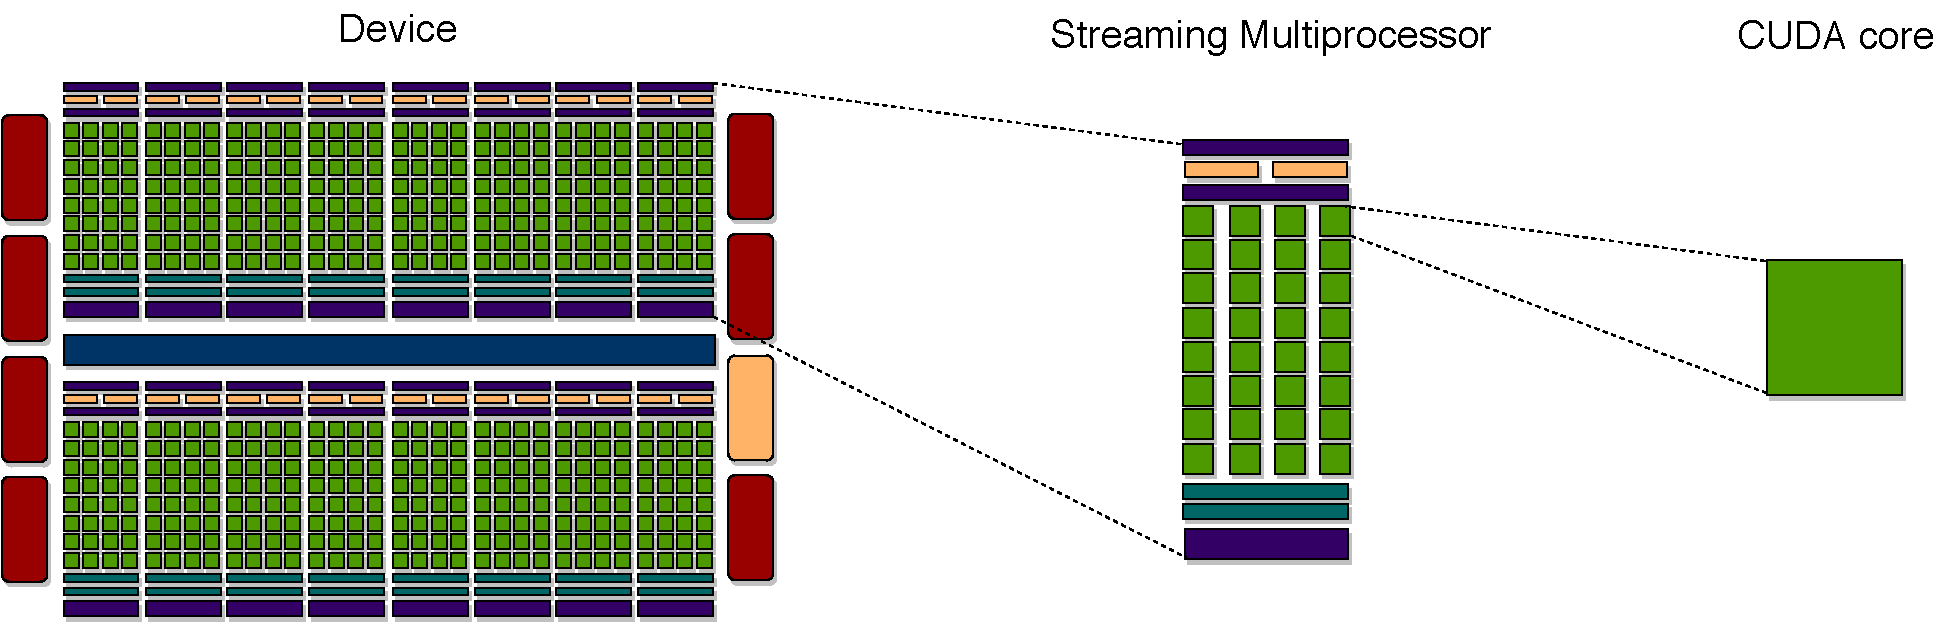
\includegraphics[width=0.9\textwidth]{fig/GPU-diagram1.pdf}

\end{frame}
\begin{frame}[noframenumbering]{Apéndice}
\framesubtitle{Arquitectura LeNet}

\centering
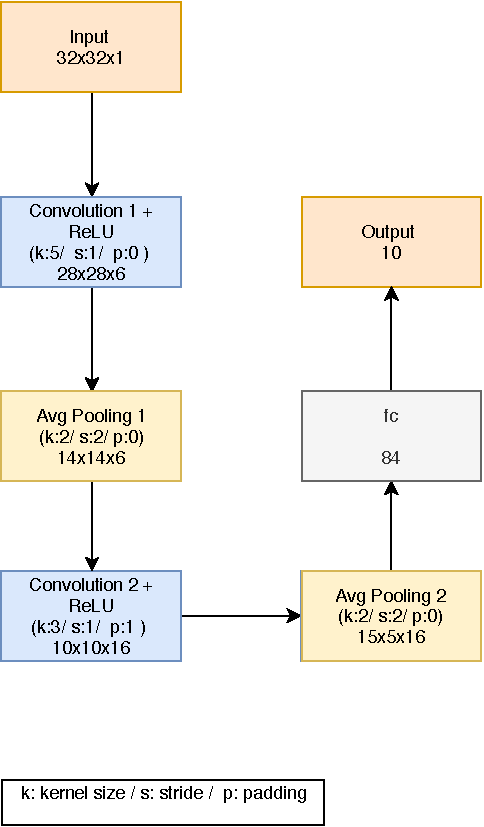
\includegraphics[width=0.35\textwidth]{anexo/lenet.pdf}

\end{frame}
\begin{frame}[noframenumbering]{Apéndice}
\framesubtitle{Modos de energía Jetson TX2}
\centering
\resizebox{0.9\linewidth}{!}{


\begin{table}[]
\centering

\begin{tabular}{lccccc}
\toprule
Modo                     & 0 & 1  & 2     & 3 & 4   \\ \midrule
Nombre                  & Max-N      & Max-Q      & Max-P Core-All & Max-P ARM  & Max-P Denver \\ 
Denver 2                & 2          & 0          & 2              & 0          & 1            \\ 
Frecuencia {[}GHz{]}     & 2          & -          & 1.4            & -          & 2            \\ 
ARM A57                  & 4          & 4          & 4              & 4          & 1            \\ 
Frec. {[}GHz{]}     & 2.0        & 1.2        & 1.4            & 2          & 0.3          \\ 
Frec. GPU {[}GHz{]} & 1.3        & 0.85       & 1.12           & 1.12       & 1.12         \\ 
\bottomrule
\end{tabular}

\end{table}
}

\end{frame}


\begin{frame}[noframenumbering]{Apéndice}
\framesubtitle{Modos de energía Jetson AGX Xavier}
\centering
\resizebox{0.9\linewidth}{!}{



\begin{table}[]

\centering
\begin{tabular}{lccccccc}
\toprule
Modo                      & 0 & 1 & 2 & 3 & 4 & 5 & 6 \\ \midrule
Power budget {[}W{]}      & n/a        & 10         & 15         & 30         & 30         & 30         & 30         \\ 
Num CPUs                    & 8          & 2          & 4          & 8          & 6          & 4          & 2          \\ 
Max freq CPU {[}MHz{]}    & 2265.6     & 1200       & 1200       & 1200       & 1450       & 1780       & 2100       \\ 
GPU TPC                   & 4          & 2          & 4          & 4          & 4          & 4          & 4          \\ 
Max freq GPU {[}MHz{]}    & 1337       & 520        & 670        & 900        & 900        & 900        & 900        \\ 
DLA Cores                 & 2          & 2          & 2          & 2          & 2          & 2          & 2          \\ 
Max freq DLA {[}MHz{]}    & 1395.2     & 550        & 750        & 1050       & 1050       & 1050       & 1050       \\ 
VA cores                  & 2          & -          & 1          & 1          & 1          & 1          & 1          \\ 
Max freq VA {[}MHz{]}     & 1088       & -          & 500        & 760        & 760        & 760        & 760        \\ 
Max freq Memory {[}MHz{]} & 2133       & 1066       & 1333       & 1600       & 1600       & 1600       & 1600       \\ 
\bottomrule
\end{tabular}

\end{table}
}
\end{frame}

\begin{frame}[noframenumbering]{Apéndice}
\framesubtitle{Trabajo Futuro}

\begin{itemize}
    \item Revisar optimizaciones para los sistemas Jetson con TensorRT de Nvidia. 
    \item Optimizaciones a nivel de funciones de cuDNN, con herramientas como $\mu$-cuDNN. 
     \item Realizar una evaluación más profunda del consumo de energía en los sistemas Jetson, considerando las limitaciones de las baterías que alimentan el sistema total, es decir, incluyendo dron y periféricos necesarios.
\end{itemize}
\end{frame}


